\section{Model Interpretability and the Role of Temperature}

\subsection{Analysis Objectives}

In drug discovery and process design, an accurate model without transparent decision logic will struggle to earn a medicinal chemist's trust, let alone guide molecular modification or process changes. This chapter addresses two mechanistic questions: the feature attribution of ExtraTrees--TabPFN and the local corrections made by TabPFN, and the physical causal link between temperature and solubility.

\subsection{Structural Contributions in SOLAR-H}

SOLAR-H is white-box by construction. From Eq.~\eqref{eq:v2-solar} the output is a linear superposition of two terms:
\begin{equation}
\widehat y_i = \underbrace{\widehat b(z_c)}_{\text{structural constant}} + \underbrace{\gamma \cdot \tau_i \cdot \left( u_c^\top \widehat\beta \right)}_{\text{structure-modulated temperature response}}.
\end{equation}
For any fixed combination $c$ the temperature derivative is constant, $\frac{\partial \widehat y}{\partial T} = \frac{\gamma u_c^\top \widehat\beta}{s_T}$. In the full development deployment, the nested validation selects the high-damping gain $\gamma = 0$, so the model degenerates to a structural-baseline prediction and avoids extrapolation drift from temperature noise on unseen parents. With a non-zero gain on the training folds, $\widehat\beta$ reveals how molecular-weight differences and polarity mismatch steer the endothermic slope.

\subsection{Feature Attribution}\label{sec:deployment-explanations}

For the nonlinear ExtraTrees--TabPFN deployed model, we combine game-theoretic Shapley values with local branch contributions in a two-pronged attribution.

\subsubsection{TreeSHAP Global Feature-Group Attribution}
For the ExtraTrees branch we use the tree-path-dependent TreeSHAP algorithm\cite{treeshap2020}, drawing 227 explanation samples that evenly cover the chemical space of the 128 development parents. TreeSHAP satisfies the local-accuracy axiom to floating-point precision (reconstruction bias below $1.3\times10^{-13}$), with a background expectation of $-1.1632$.

The 665 retained features fall into four groups: drug descriptors, solvent descriptors, temperature, and explicit intermolecular interactions. Each group's signed attribution is averaged equally over the 128 parents (Figure~\ref{fig:deployment-explanations}A).

\begin{figure}[htbp]
\centering
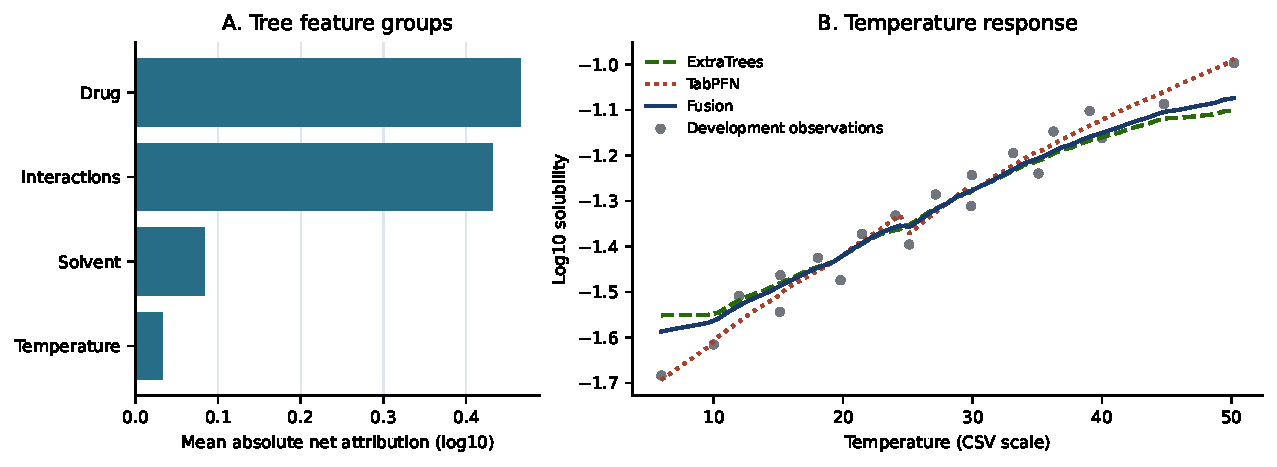
\includegraphics[width=\linewidth]{deployment_explanations.pdf}
\caption{Feature attribution and dynamic temperature response of the deployed model. \textbf{A} parent-equal absolute net attribution of the four feature groups; \textbf{B} predicted curve for the lovastatin--butyl acetate combination over its observed temperature window (markers are measurements, the solid line is the blend, dashed lines are the single branches).}
\label{fig:deployment-explanations}
\end{figure}

The attribution is chemically interpretable. Drug descriptors (mean absolute attribution 0.466) and explicit interaction features (0.432) contribute most to the predictions. This matches solution physicochemical principles: drug molecules are large and complex (molecular weights usually 200--800), and their lattice energy and solid-state cohesion are a barrier to dissolution; the explicit solute--solvent interactions (polarity matching and hydrogen bonding) then decide whether solvation can overcome that lattice energy. Solvent descriptors (0.084) and temperature (0.033) only fine-tune the prediction. Because the solvent library is small (49 common industrial solvents) and its structures are regular, the solvent's standalone contribution is concentrated and acts mostly as a conditional perturbation on the structural baseline.

\subsubsection{TabPFN's Local Branch Calibration}
To see how TabPFN cooperates with ExtraTrees, Table~\ref{tab:deployment-examples} picks two real cases where the TabPFN correction $\Delta_{\mathrm{PFN}} = 0.25 (f_{\mathrm{PFN}} - f_{\mathrm{ET}})$ takes extreme values in opposite directions.

\begin{table}[htbp]
\centering\small
\setlength{\tabcolsep}{4pt}
\caption{Two representative cases of TabPFN's bidirectional calibration of the ExtraTrees branch (both in acetone).}
\label{tab:deployment-examples}
\begin{tabular}{lrrrrrr}
\toprule
Drug (row) & Temperature ($^\circ\text{C}$) & Measured & ExtraTrees & TabPFN & Blend & Correction $\Delta_{\mathrm{PFN}}$ \\
\midrule
Erythritol (row 23) & 13.2 & $-2.692$ & $-2.495$ & $-2.716$ & $-2.551$ & $-0.055$ (down) \\
4-hydroxyphenylglycine Dane salt (row 3) & 70.2 & $-1.843$ & $-1.927$ & $-1.847$ & $-1.907$ & $+0.020$ (up) \\
\bottomrule
\end{tabular}
\end{table}

The two cases illustrate the ensemble's adaptive calibration. For erythritol, ExtraTrees is pulled toward the statistical mean of polyols at room temperature and predicts $-2.495$, a clear overestimate of the measured $-2.692$; TabPFN, attending over continuous space, recognises the insolubility of a highly polar small molecule in a low-polarity solvent and predicts $-2.716$, driving the blend down to $-2.551$ and cutting the error sharply. For the Dane salt, ExtraTrees is conservative ($-1.927$), while TabPFN picks up the thermodynamic solubilisation at $70.2^\circ\text{C}$ and predicts $-1.847$, nudging the blend up to $-1.907$, close to the measured $-1.843$. TabPFN thus applies corrections in opposite directions across different chemical spaces, drawing on its rich prior-manifold representation.

\subsection{Dynamic Temperature Response}

To check physical plausibility under continuous temperature change, we fix the lovastatin--butyl acetate system (20 dense temperature points in the development set, spanning $[5.95^\circ\text{C}, 50.2^\circ\text{C}]$) and scan the temperature densely (Figure~\ref{fig:deployment-explanations}B).

The temperature scan shows different behaviours: ExtraTrees produces a staircase of piecewise segments, as expected from an axis-split tree, while the blend traces a smooth, monotone upward curve whose log-solubility rises from $-1.587$ at $5.95^\circ\text{C}$ to $-1.074$ at $50.2^\circ\text{C}$. The curve passes through the middle of the observed scatter and matches the endothermic-dissolution behaviour of most solid solutes.
